\documentclass[12pt]{article}
\usepackage{graphicx}
\usepackage{float}
\usepackage{caption}
\usepackage{subcaption}
\usepackage{fullpage}
\usepackage{lastpage}
\usepackage{fancyhdr}
\usepackage{wrapfig}
\usepackage{lipsum}
\usepackage{mathtools}
\usepackage{amsfonts}
\usepackage{enumitem}
\usepackage{amsmath}
\usepackage{listings}
\usepackage{amssymb}
\usepackage[margin=0.8in]{geometry}

\newcommand{\s}{\hspace{5pt}}
\newcommand{\half}{\frac{1}{2}}
\newcommand{\R}{\mathbb{R}}
\newcommand{\C}{\mathbb{C}}
\newcommand{\p}{\partial}
\newcommand{\mb}{\mathbf}

\newenvironment{m}{\begin{pmatrix}}{\end{pmatrix}}
\newenvironment{e}{\begin{enumerate}[label=(\alph*)]}{\end{enumerate}}

\setlength{\parindent}{0in}

\begin{document}

\title{\vspace{-5ex}Plasma Educational Notes: Two-Stream Instability\vspace{-1ex}}
\date{\vspace{-1ex}\today}
\author{Kyle Miller \& Lance Hildebrand}
\maketitle

\section*{Introduction}

A two-stream instability occurs when two species (either the same or different) in a plasma have different drift velocities. Depending on the physical parameters, modes can then arise which are unstable and grow exponentially. To begin, we derive the general dispersion relation for these instabilities.

\section*{General Dispersion Relation}

Consider two cold species, which we will generically label species 1 and species 2, each with constant drift velocity $\mb{v}_{0,1}$ and $\mb{v}_{0,2}$ and fluctuating velocity $\tilde{\mb{v}}_1$ and $\tilde{\mb{v}}_2$, respectively. The linearized Navier-Stokes equation for each species is then

\begin{align*}
\frac{d}{d t} \tilde{\mb{v}}_s &= \frac{\p}{\p t} \tilde{\mb{v}}_s + \mb{v}_{0,s} \cdot \nabla \tilde{\mb{v}}_s = \frac{q_s}{m_s} \tilde{\mb{E}}.
\end{align*}

In addition, the continuity equation for each species is

\begin{align*}
\frac{\p}{\p t} \tilde{n}_s + n_{0,s} \nabla \cdot \tilde{\mb{v}}_s + \mb{v}_{0,s} \cdot \nabla \tilde{n}_s &= 0.
\end{align*}

Poisson's equation then yields

\begin{align*}
\nabla \cdot \tilde{\mb{E}} = 4\pi \sum_{s}q_s \tilde{n}_s.
\end{align*}

If we assume a plane wave solution of the form $\tilde{\mb{E}} = \mb{E}_0 e^{i(\mb{k} \cdot \mb{r} - \omega t)}$, then the dynamical equation turns into

\begin{align*}
(-i\omega + i \mb{k} \cdot \mb{v}_{0,s})\tilde{\mb{v}}_s = \frac{q_s}{m_s} \tilde{\mb{E}} \\
\Rightarrow \tilde{\mb{v}}_s = \frac{q_s \tilde{\mb{E}}}{i m_s (-i\omega + i \mb{k} \cdot \mb{v}_{0,s})}.
\end{align*}

Similarly, the continuity equation can be rewritten as

\begin{align*}
-i\omega \tilde{n}_s + i n_{0,s} \mb{k} \cdot \tilde{\mb{v}}_s + i \mb{k} \cdot \mb{v}_{0,s} \tilde{n}_s = 0 \\
\Rightarrow \tilde{n}_s = \frac{n_{0,s} \mb{k} \cdot \tilde{\mb{v}}_s}{\omega - \mb{k} \cdot \mb{v}_{0,s}} = \frac{-q_s n_{0,s} \mb{k} \cdot \tilde{\mb{E}}}{i m_s (\omega - \mb{k} \cdot \mb{v}_{0,s})^2}.
\end{align*}

If we substitute this expression for $\tilde{n}_s$ into Poisson's equation, after rearranging we find that

\begin{align*}
\left(1 - \sum_s\frac{\omega_{p,s}^2}{(\omega - \mb{k} \cdot \mb{v}_{0,s})^2}\right)i \mb{k} \cdot \tilde{\mb{E}} = 0.
\end{align*}

Recognizing that $\nabla \cdot \tilde{\mb{D}} = \nabla \cdot (\epsilon \tilde{\mb{E}}) = \epsilon \mb{k} \cdot \tilde{\mb{E}}$, the term in parenthesis is then our dielectric constant. Setting this equal to zero gives the dispersion relation as

\begin{align*}
1 - \frac{\omega_{p,1}^2}{(\omega - \mb{k} \cdot \mb{v}_{0,1})^2} - \frac{\omega_{p,2}^2}{(\omega - \mb{k} \cdot \mb{v}_{0,2})^2} = 0.
\end{align*}

This equation can be used for various types of two-stream instabilities, for which the parameters $\omega_{p,s}$ and $\mb{v}_{0,s}$ can be adjusted. Following are several specific cases of the two-stream instability.

\section*{Farley-Buneman Instability}
Consider a stationary background of ions with the electron plasma moving with a constant drift velocity $\mb{v}_0$. This could be produced, for example, by a current-carrying plasma. Then the dispersion relation is reduced to

\begin{align*}
1 = \omega_{pe}^2 \left(\frac{m_e/m_i}{\omega^2} + \frac{1}{(\omega - \mb{k} \cdot \mb{v}_0)^2}\right).
\end{align*}

This quartic equation can be cast into a simpler form by defining $x \equiv \omega/\omega_{pe}$ and $\alpha \equiv \mb{k} \cdot \mb{v}_0/\omega_{pe}$ to get

\begin{align*}
1 = \frac{m_e/m_i}{x^2} + \frac{1}{(x-\alpha)^2}.
\end{align*}

\subsection*{Parameters}

From the above equation, it is seen that the two free parameters in the problem are the ratio of electron to ion mass, $m_e/m_i$, and $\alpha = \mb{k} \cdot \mb{v}_0/\omega_{pe}$, or simply the ratio $\mb{k} \cdot \mb{v}_0/n_0$.

\subsection*{Solution to the dispersion relation}

If we define the right-hand side of the equation as

\begin{align*}
f(x) = \frac{m_e/m_i}{x^2} + \frac{1}{(x-\alpha)^2},
\end{align*}

then we seek for solutions to $f(x) = 1$. In Fig.~\ref{fig:Buneman}, we see that two of the roots for $\omega$ are always real, and the other two roots may be real or complex depending on the value of $\alpha$. To find when the $\omega$ roots begin to be complex, we seek to minimize $f(x)$. Setting $\frac{m_e}{m_i} \approx \frac{1}{1836}$ and solving $f'(x)=0$ yields $x_{min} \approx 0.75\alpha$. Then setting $f(x_{min}) \geq 1$ means that to have complex roots we need $\alpha \lesssim 1.12$. This is shown in the red curve in Fig.~\ref{fig:Buneman}.

\begin{figure}
	\centering
	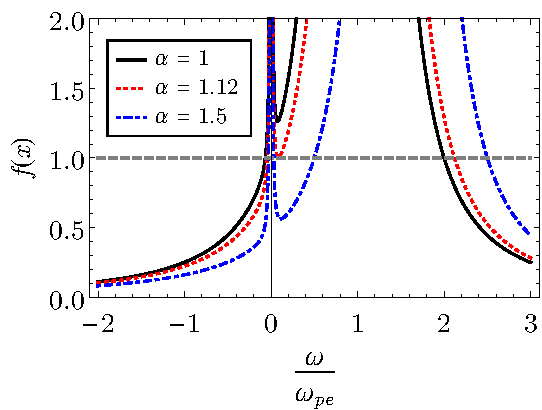
\includegraphics[width=0.5\textwidth]{two_stream_disp}
	\caption{\label{fig:Buneman} Plot from the dispersion relation for various values of $\alpha$. Modes occur where $f(x)=1$.}
\end{figure}

%To find the growth rate, we manipulate the dispersion relation to obtain

%\begin{align*}
%x^2(x-\alpha)^2-\frac{m_e}{m_i}(x-\alpha)^2-x^2 = 0.
%\end{align*}

If we let $\omega = \omega_R+i \omega_I$, then solving for $\omega_I$ gives the growth rate. The real and imaginary parts of the frequency are shown in Fig.~\ref{fig:omega_roots}.

\begin{figure}
	\centering
	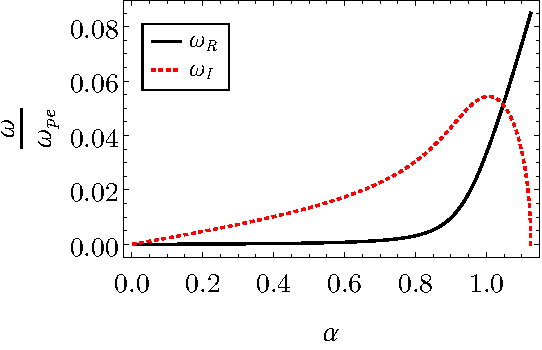
\includegraphics[width=0.5\textwidth]{omega_roots}
	\caption{\label{fig:omega_roots} Real and imaginary parts of the frequency as a function of $\alpha$. The most unstable mode is observed for $\alpha \approx 1$.}
\end{figure}

\section*{Weak Cold Beam Instability}
Consider a stationary electron-ion plasma with a fast, weak beam of electrons passing through it. Here ``fast'' implies $v_b \gg \bar{v}_e, \bar{v}_i$, ``weak'' implies $n_b/n_0 \ll 1$, and ``cold'' implies $v_b \gg \bar{v}_b$. Since $\omega_{pi} \ll \omega_{pe}$, we neglect the ion contribution to the dispersion relation and obtain

\begin{align*}
1 = \frac{\omega_{pe}^2}{\omega^2} + \frac{\omega_{pb}^2}{(\omega-\mb{k} \cdot \mb{v}_b)^2}.
\end{align*}

Defining $x \equiv \omega/\omega_{pb}$ and $\alpha \equiv \mb{k} \cdot \mb{v}_b/\omega_{pb}$, along with recognizing that $\omega_{pe}^2/\omega_{pb}^2 = n_0/n_b$, we then get that

\begin{align*}
1 = \frac{n_0/n_b}{x^2} + \frac{1}{(x-\alpha)^2}.
\end{align*}

\subsection*{Parameters}

From the above equation, it is seen that the two free parameters in the problem are the ratio of background to beam density, $n_0/n_b$, and $\alpha = \mb{k} \cdot \mb{v}_b/\omega_{pb}$, or simply the ratio $\mb{k} \cdot \mb{v}_b/n_b$.

\subsection*{Solution to the dispersion relation}

Analysis proceeds exactly as in the discussion for the Farley-Buneman instability, but now $n_0/n_b \gg 1$. This results in complex values of $\omega$ for much larger allowable values of $\alpha$ than before. For example, with $n_0/n_b = 2000$, $\omega$ is complex for $\alpha \lesssim 50$.

\section*{References}
[1] N. A. Krall and A. W. Trivelpiece, ``Principle of Plasma Physics,'' McGraw Hill, New York, 1973.

\end{document}
